\section{Evaluation}\label{sec:eval}

\begin{figure*}[t]
  \centering
  \begin{subfigure}[t]{0.48\textwidth}
    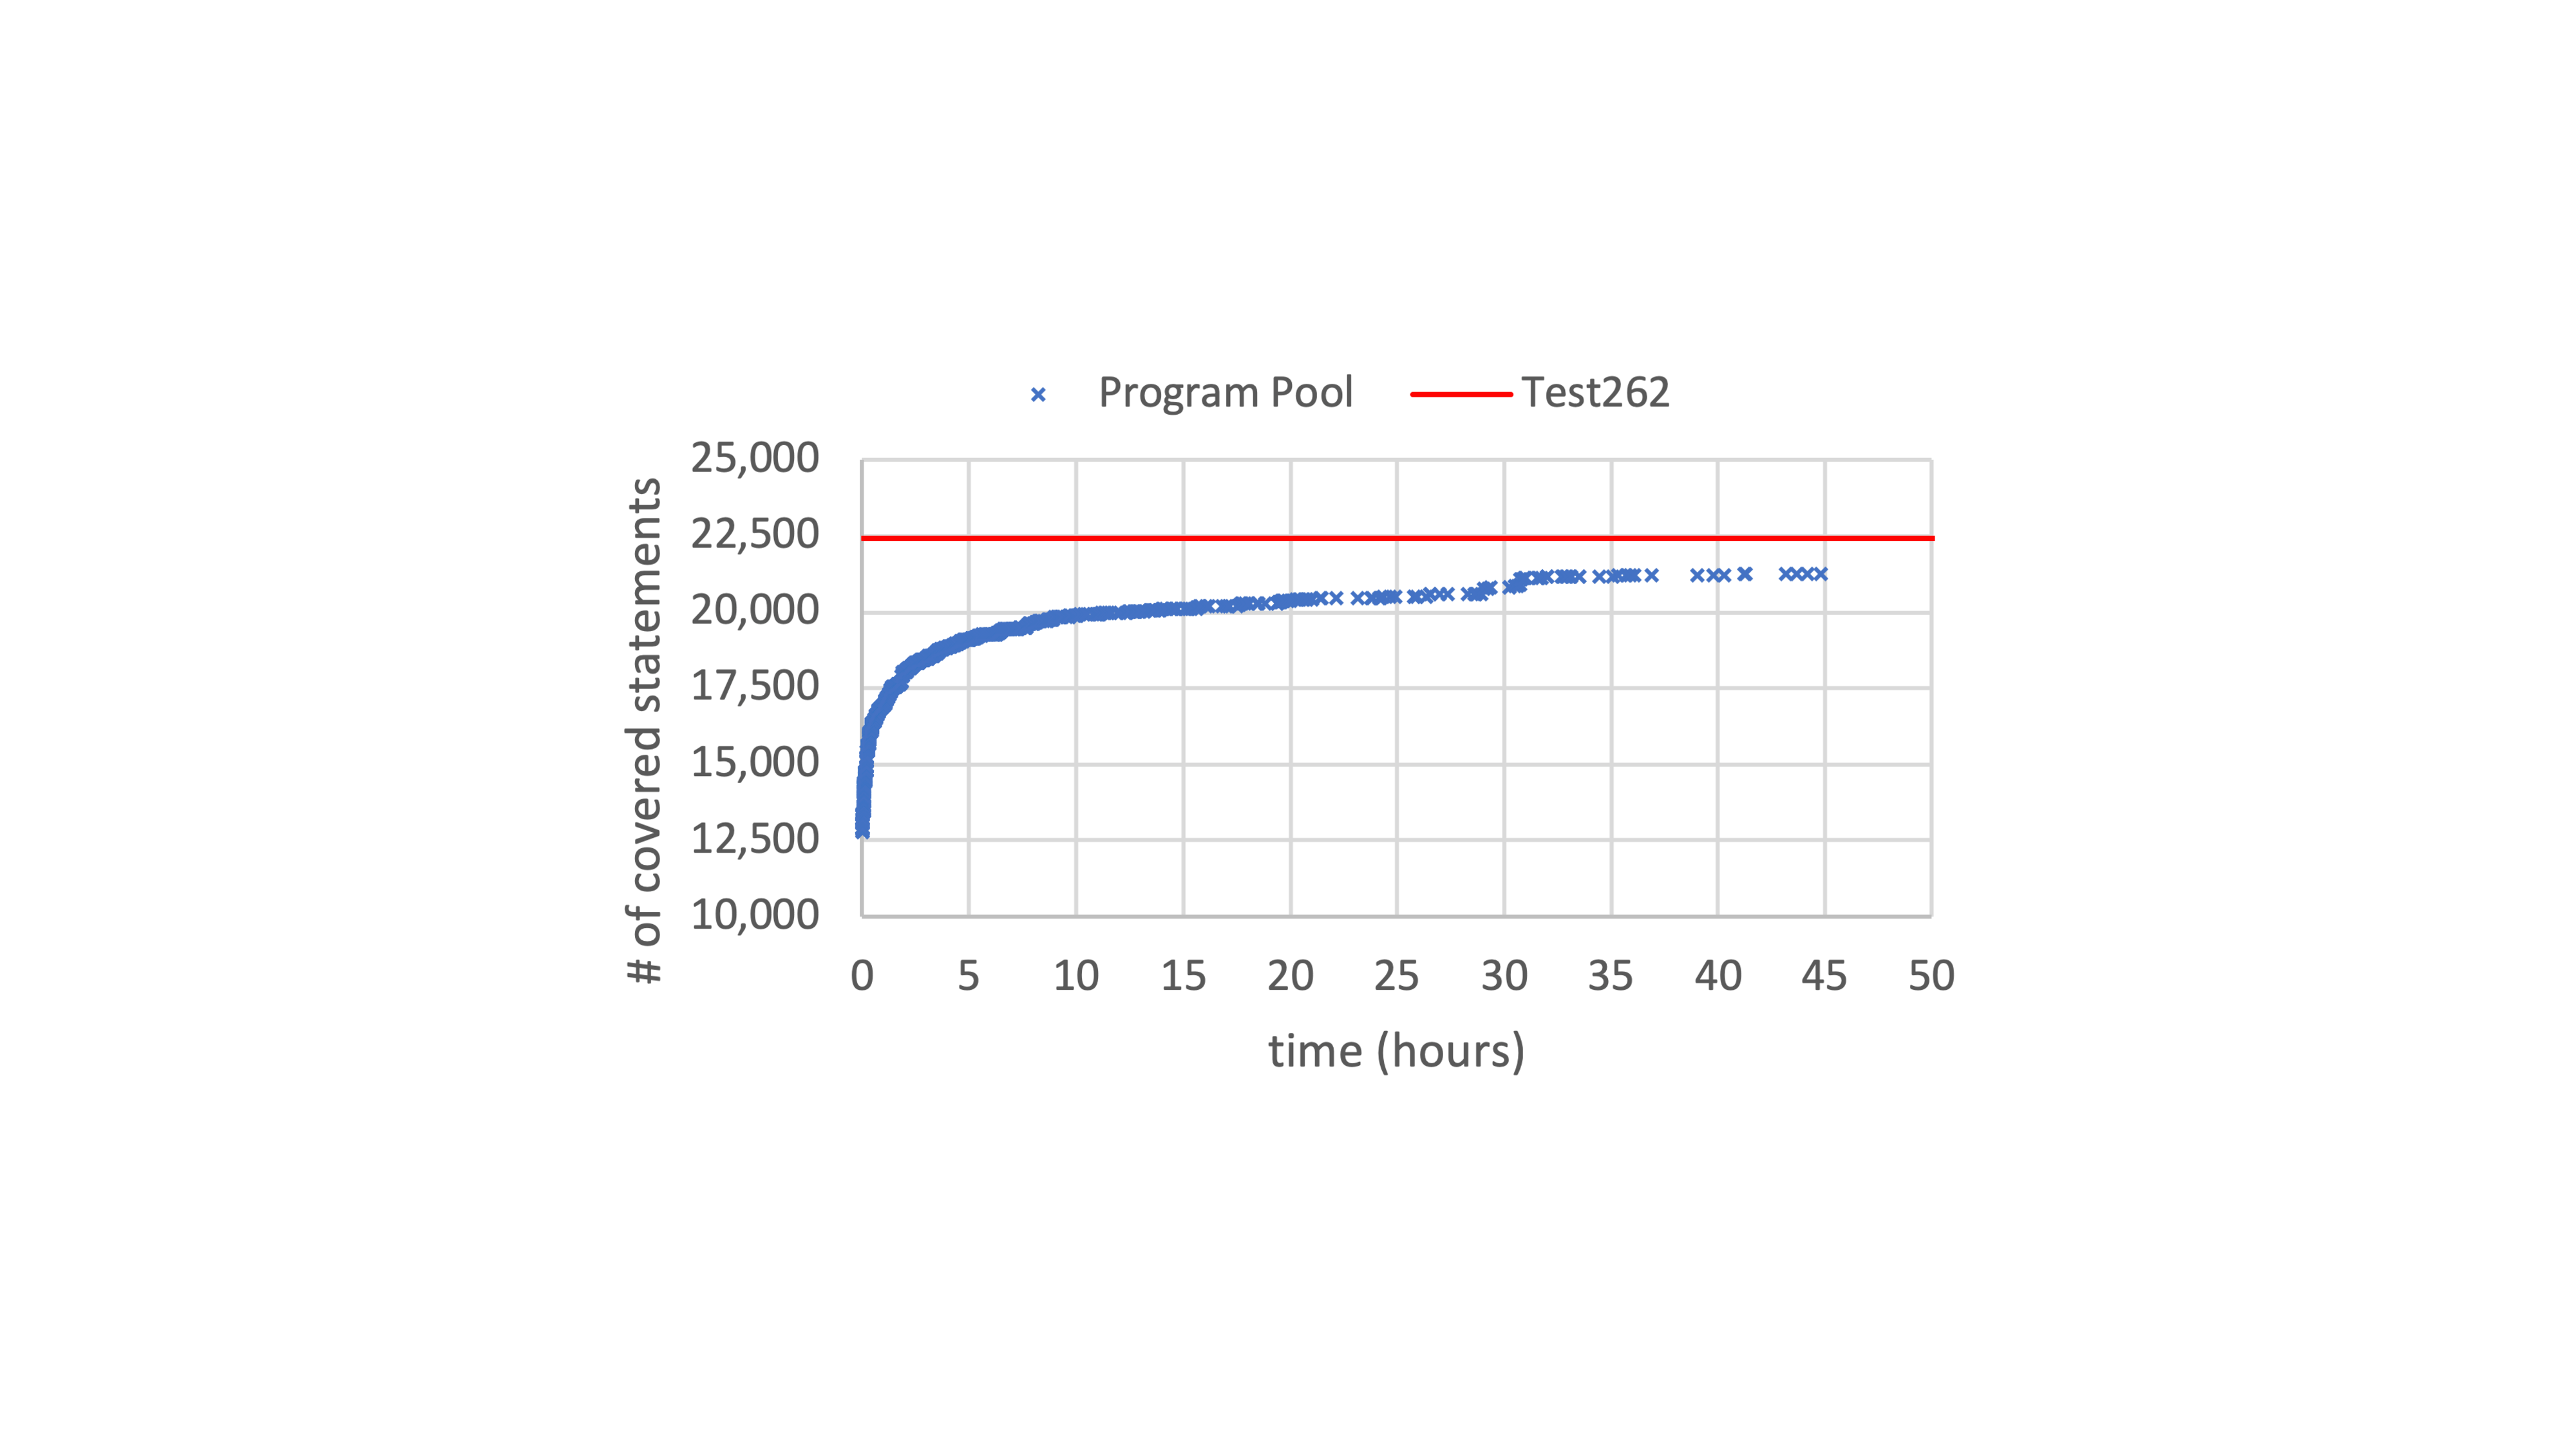
\includegraphics[width=\textwidth]{img/stmt-coverage.pdf}
    \caption{The statement coverage}
    \label{fig:stmt-coverage}
  \end{subfigure}
  \quad
  \begin{subfigure}[t]{0.48\textwidth}
    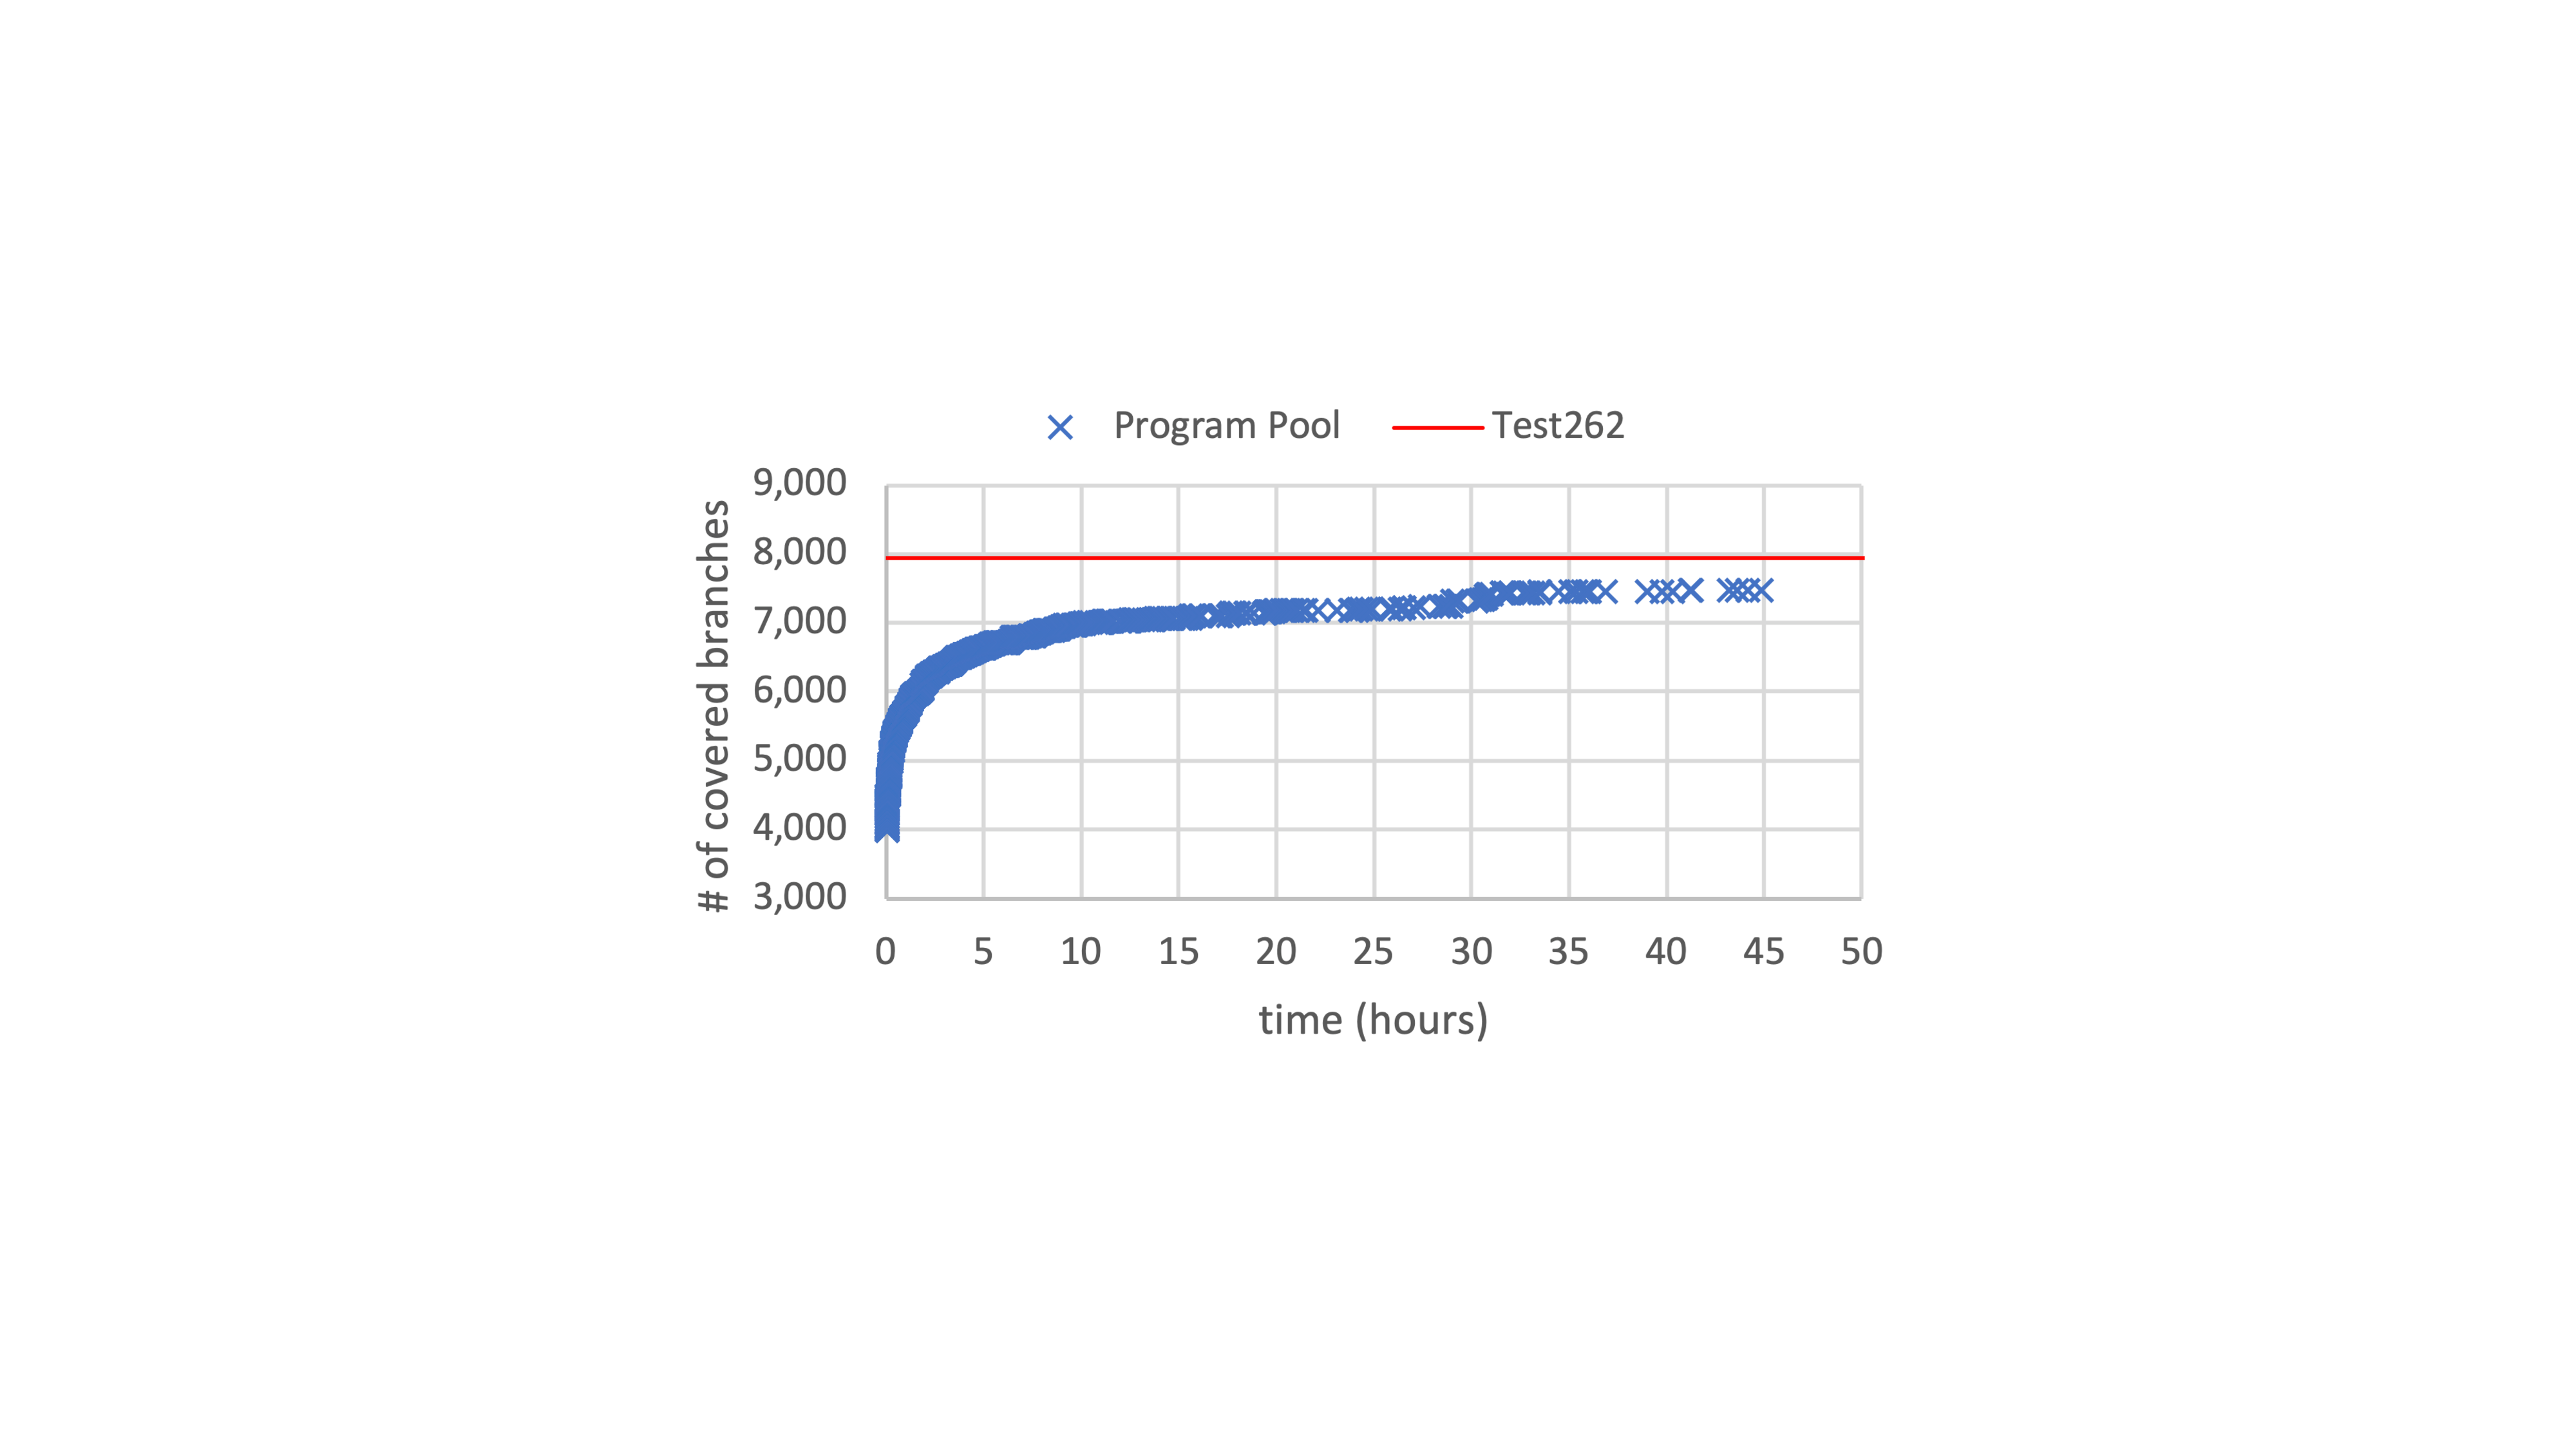
\includegraphics[width=\textwidth]{img/branch-coverage.pdf}
    \caption{The branch coverage}
    \label{fig:branch-coverage}
  \end{subfigure}
  \caption{The semantics coverage changes during the test generation phase}
  \label{fig:sem-coverage}
  \vspace*{-1em}
\end{figure*}

To evaluate $\tool$ that performs the $N$+1-differential testing of JavaScript
engines and specification, we applied our tool to four JavaScript engines that
fully support modern JavaScript features and the most recent specification,
ECMAScript 2020 (ES11, 2020).  We targeted the following four JavaScript
engines and all of them supports
ES11\footnote{https://github.com/graalvm/graaljs\#current-status}\footnote{https://bellard.org/quickjs/}\footnote{https://blog.moddable.com/blog/xs10/}\footnote{https://v8.dev/}:
\begin{itemize}
  \item \textbf{GraalJS(v20.1.0):} A JavaScript implementation built on
    GraalVM\cite{graaljs}, which is a Java Virtual Machine (JVM) based on
    HotSpot/OpenJDK developed by Oracle.
  \item \textbf{QuickJS(2020-04-12):} A small and embedded JavaScript engine developed by
    Fabrice Bellard and Charlie Gordon\cite{qjs}.
  \item \textbf{Moddable XS(v10.2.1):} A JavaScript engine at the center of the Moddable
    SDK\cite{xs}, which is a combination of development tools and runtime
    software to create applications for micro-controllers.
  \item \textbf{V8(v8.5):} The Google's open source high-performance JavaScript and
    WebAssembly engine\cite{v8}, written in C++.
\end{itemize}
To extract mechanized specification from ECMAScript, we utilize the tool
$\jiset$, which is a JavaScript IR-based semantics extraction toolchain.
automatically extracted from a given ECMAScript.  To focus on the semantics of
core JavaScript semantics, we only consider the semantics of strict mode
JavaScript codes that pass syntax checking including the EarlyError rules.  To
filter out the JavaScript codes that are not strict or fail the syntax checking,
we utilize the syntax checker of the most reliable JavaScript engine, V8.
We performed our experiments on a machine equipped with 4.0GHz Intel(R) Core(TM)
i7-6700k and 32GB of RAM (Samsung DDR4 2133MHz 8GB*4).  We evaluated our tool
based on the following four research questions:
\begin{itemize}
  \item {\bf RQ1 (Coverage of Generated Tests)} The semantics coverage compared
    to Test262, the manually written official conformance test suite for
    ECMAScript.
  \item {\bf RQ2 (Accuracy of Bug Localization)} The accuracy of bug locations
    pointed by \textsf{Bug Localizer} compared to the actual bug locations.
  \item {\bf RQ3 (Bug Detection in JavaScript Engines)} The number of bugs in
    four JavaScript engines detected by $\tool$.
  \item {\bf RQ4 (Bug Detection in ECMAScript)} The number of specification bugs
    in ES11 detected by $\tool$.
\end{itemize}


\subsection{Coverage of Generated Tests}

\begin{figure*}[t]
  \centering
  \begin{subfigure}[t]{0.48\textwidth}
    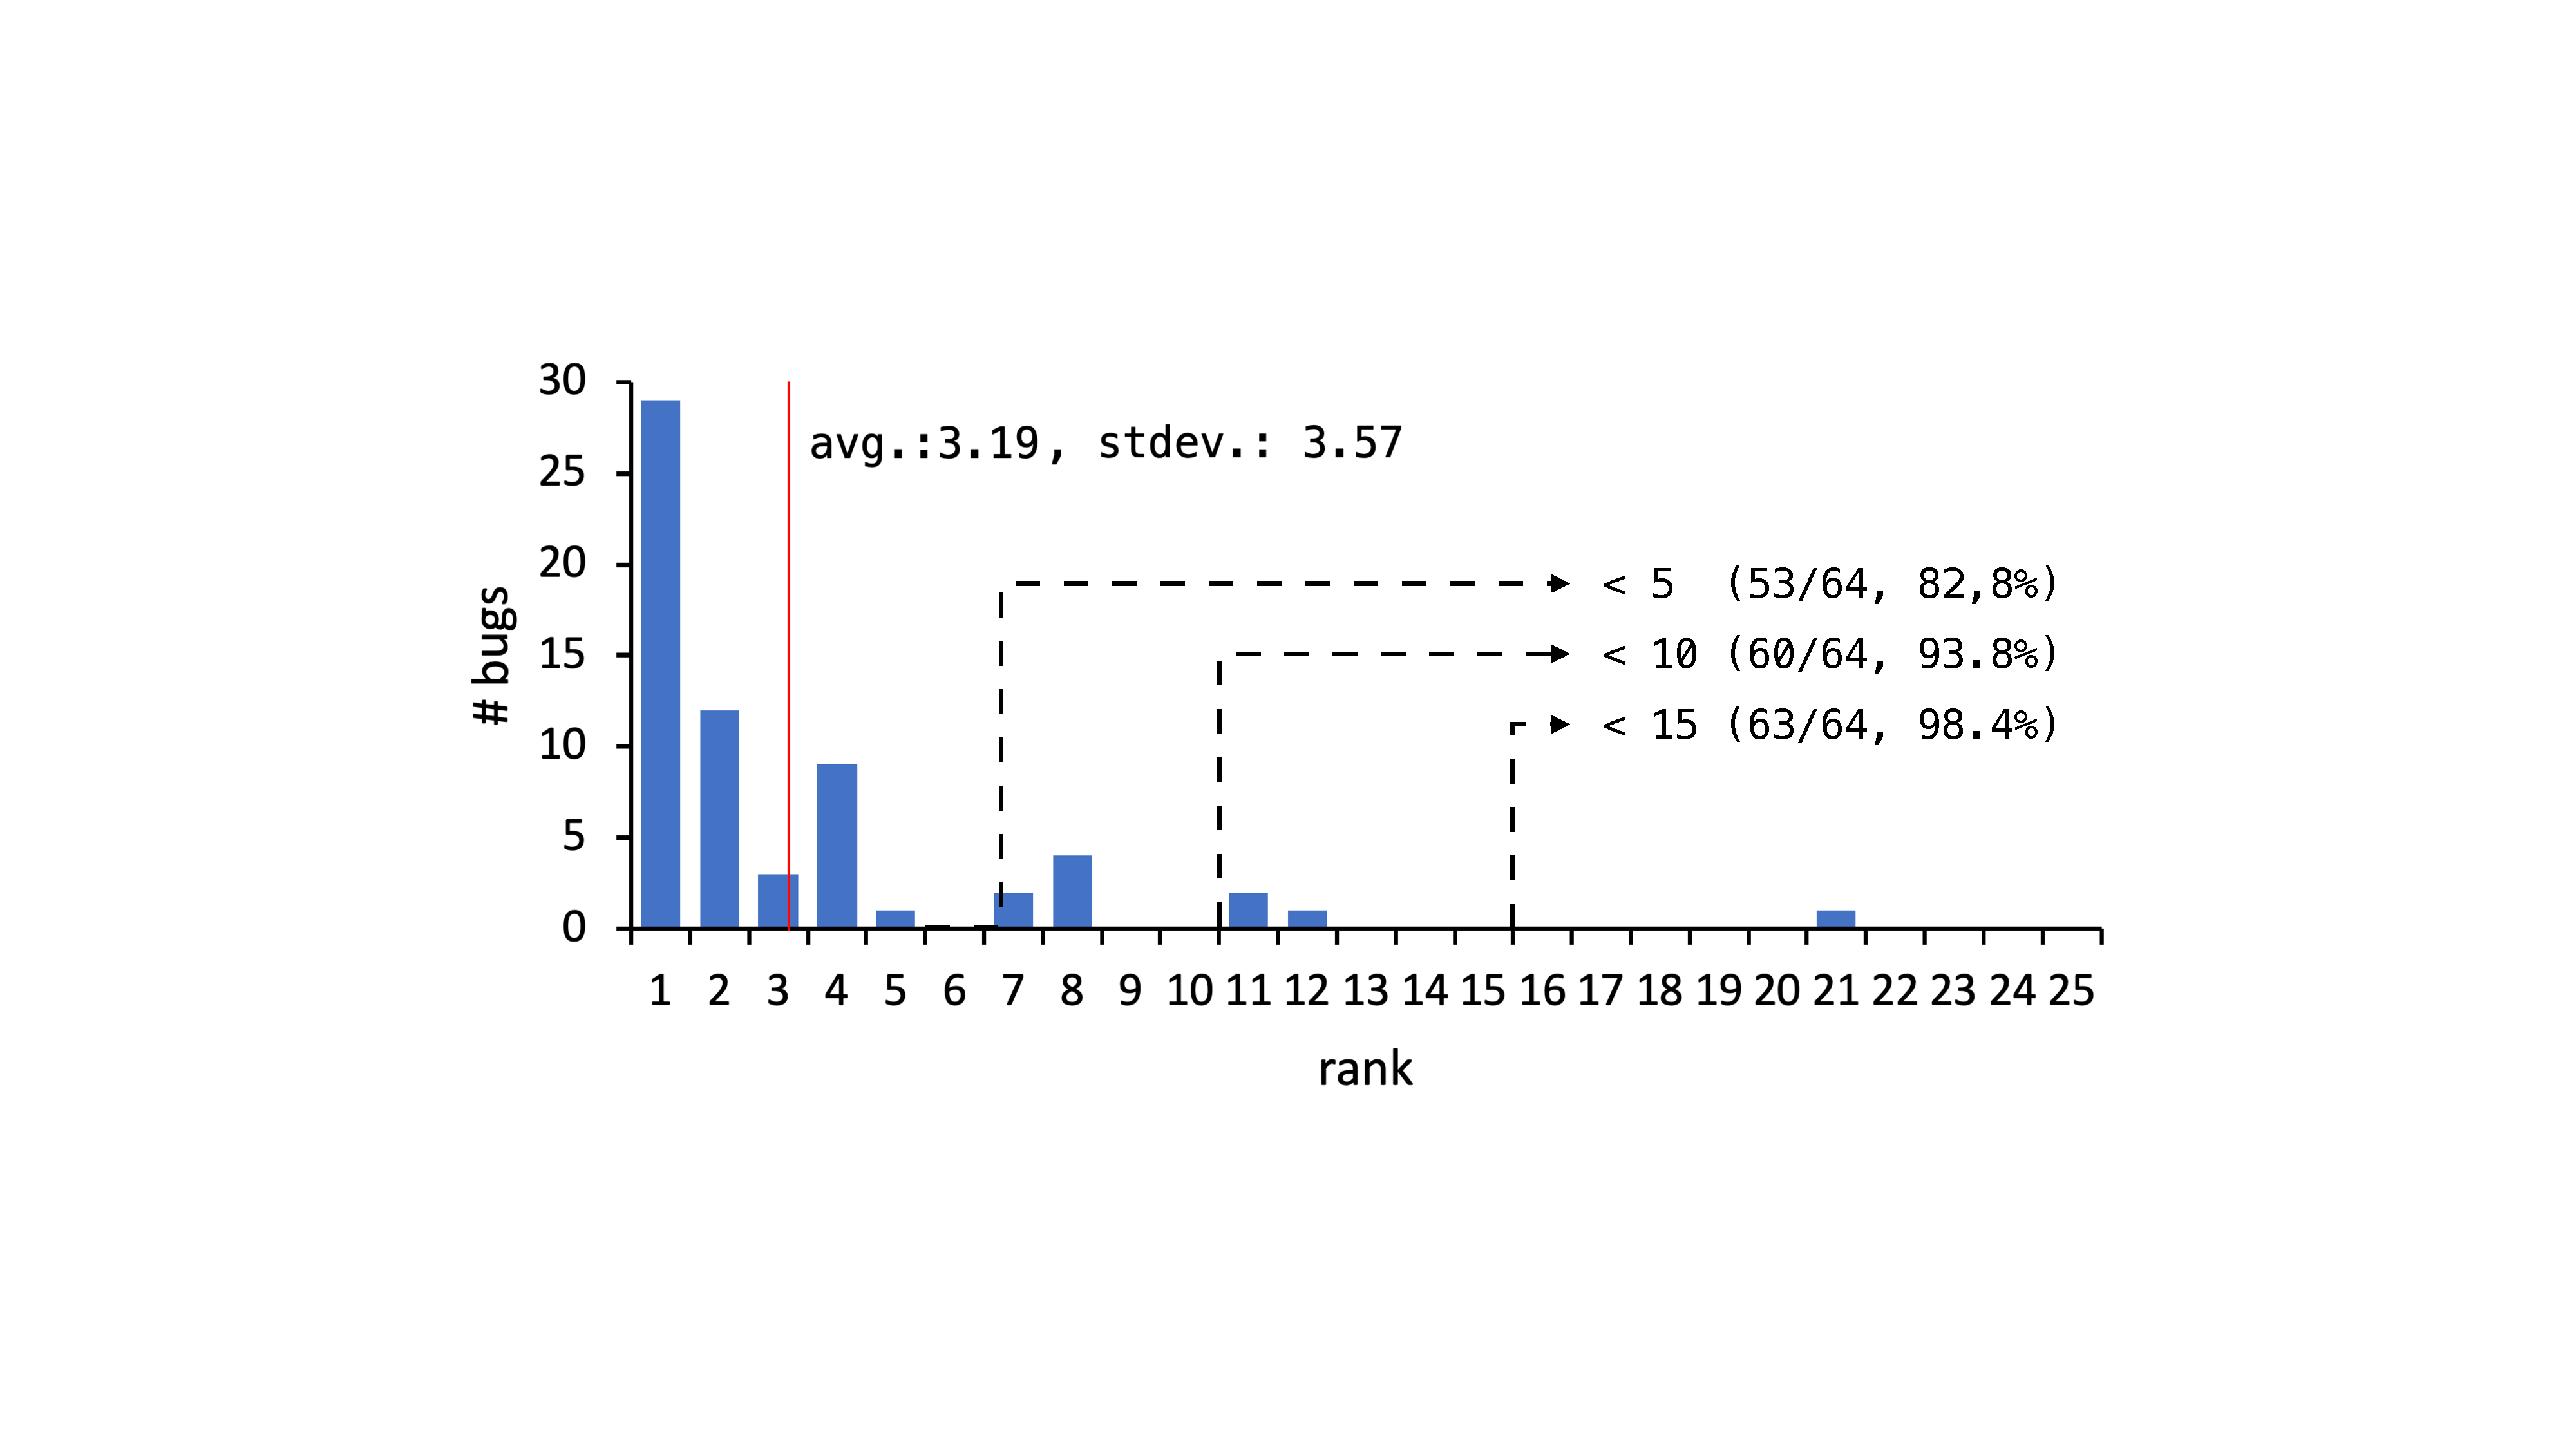
\includegraphics[width=\textwidth]{img/localize.pdf}
    \caption{Localization for algorithms}
    \label{fig:localize-algo}
  \end{subfigure}
  \begin{subfigure}[t]{0.48\textwidth}
    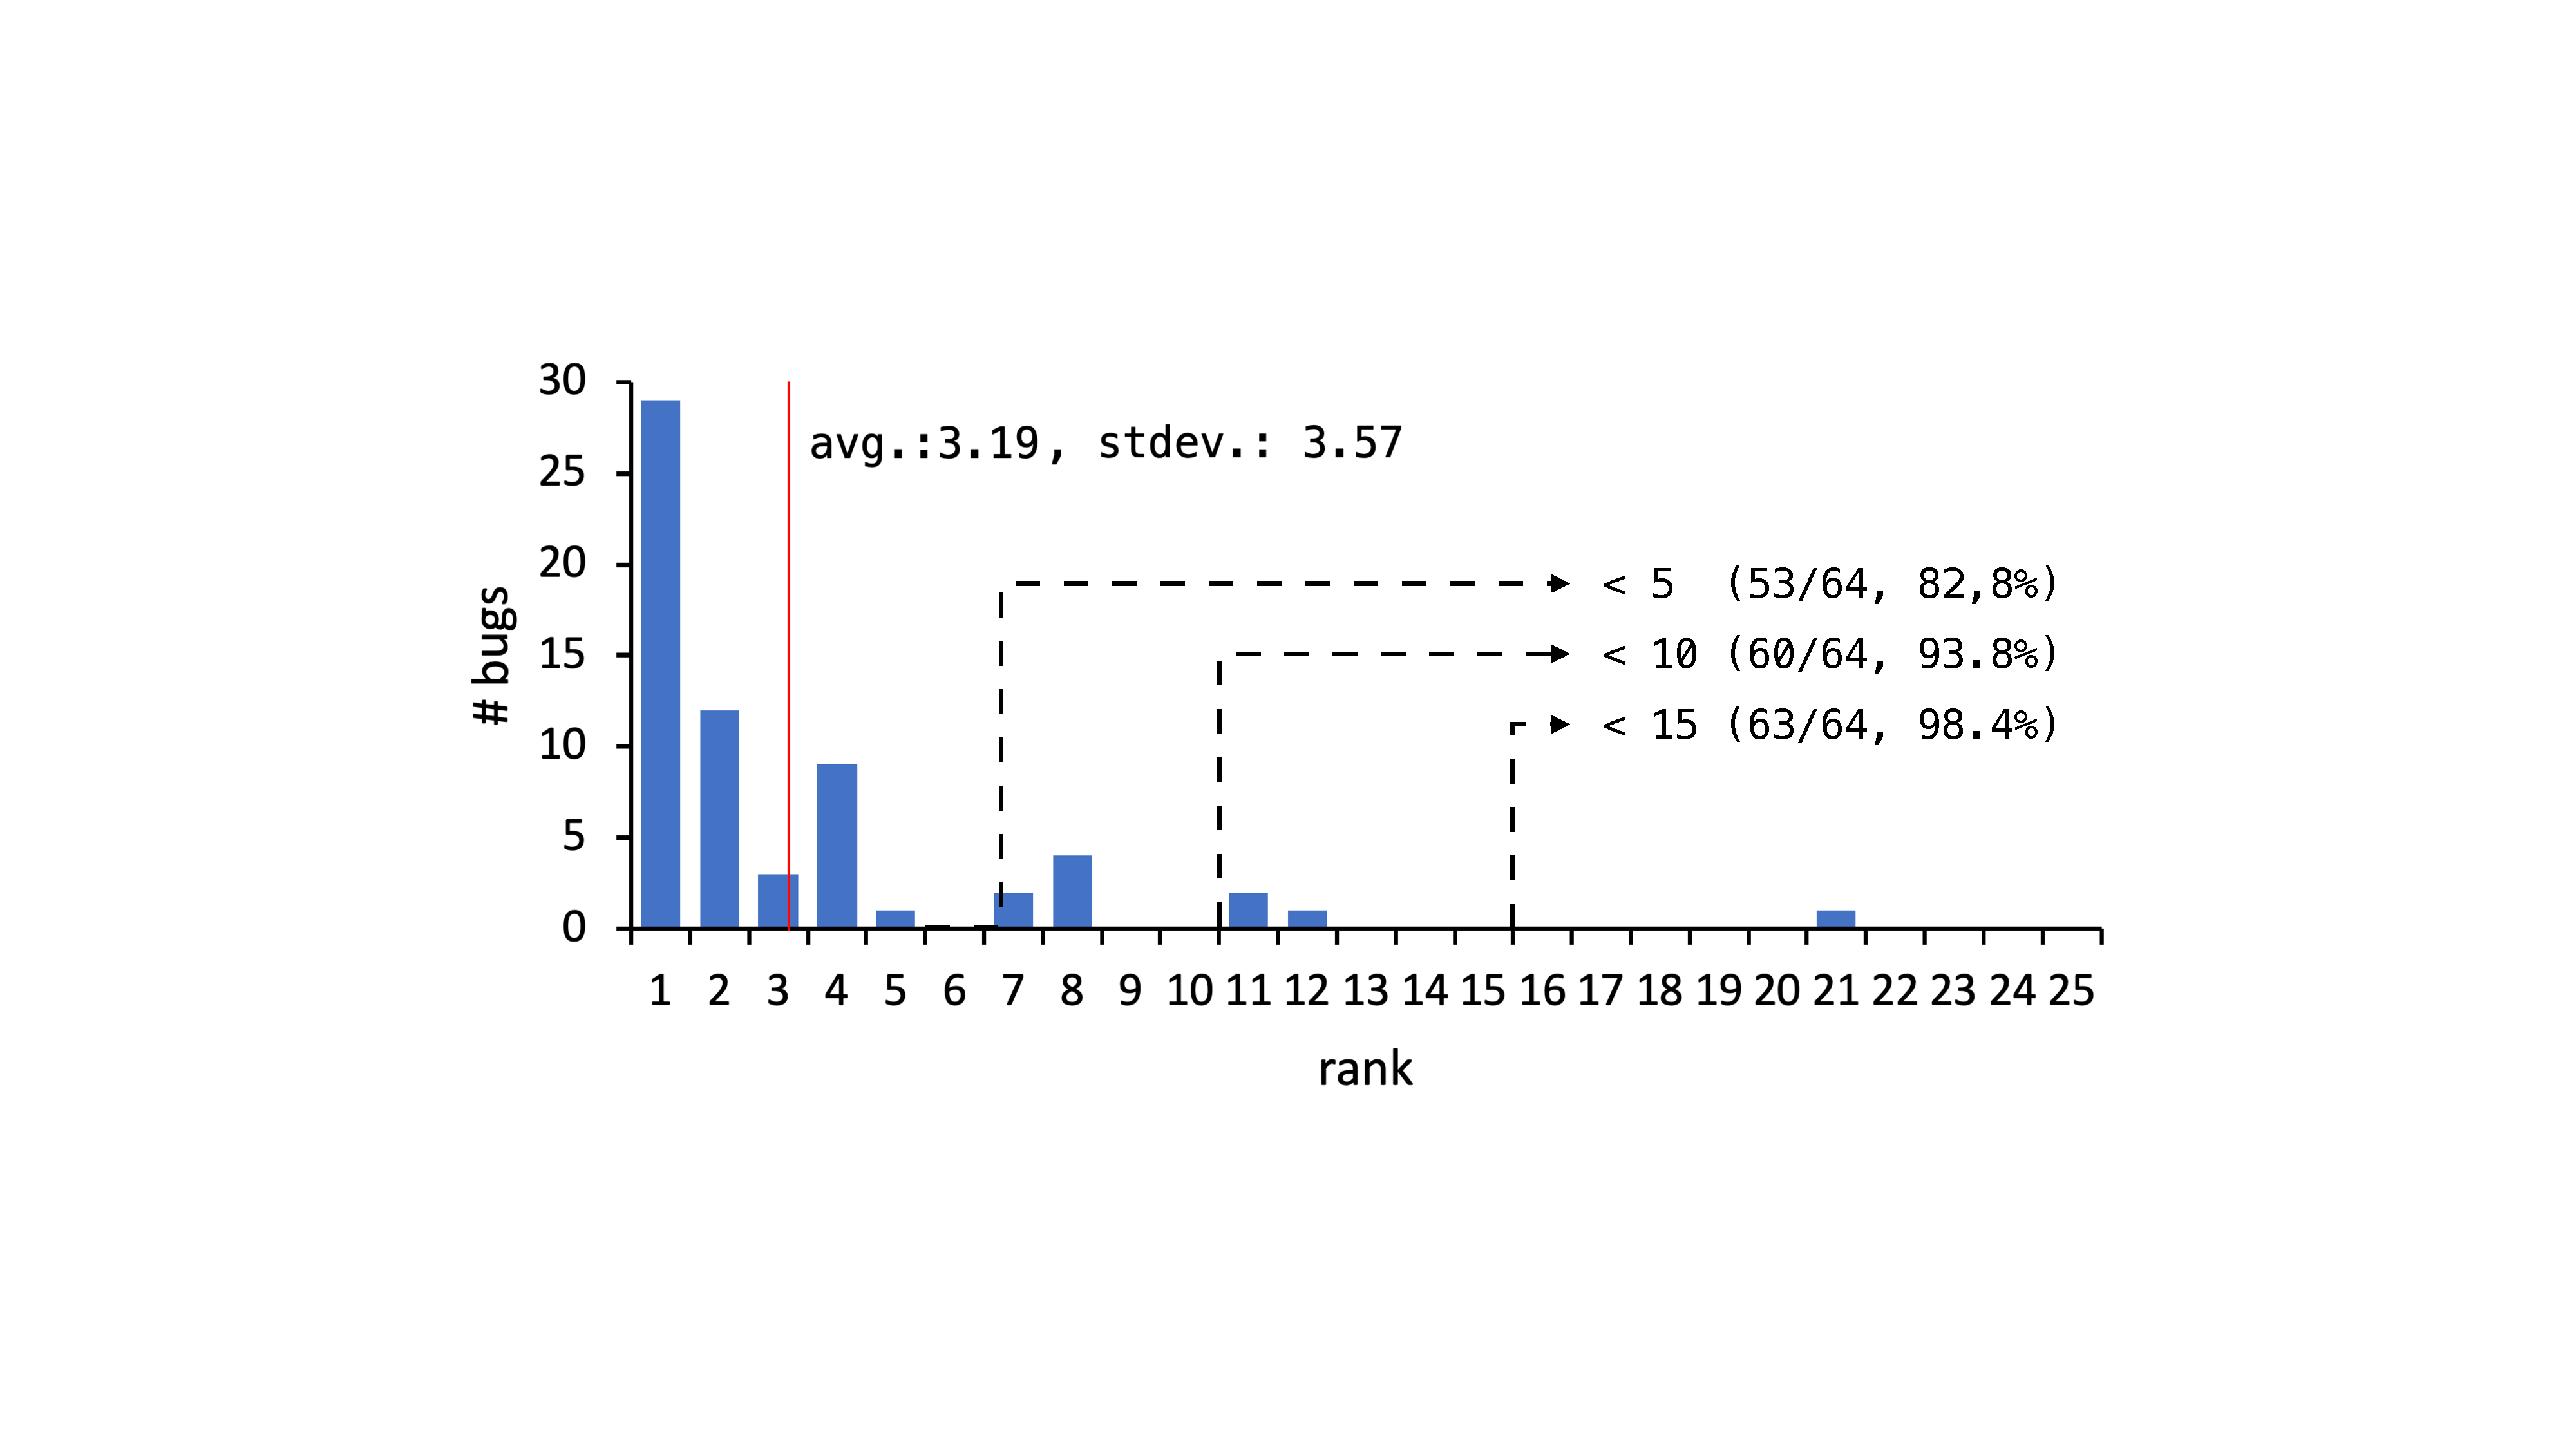
\includegraphics[width=\textwidth]{img/localize.pdf}
    \caption{Localization for algorithm steps}
    \label{fig:localize-step}
  \end{subfigure}
  \caption{Ranks of actual bug locations in results of \textsf{Bug Localizer}
    for all detected specification or engine bugs by $\tool$}
  \label{fig:localize}
  \vspace*{-1em}
\end{figure*}

For the first step, we synthesize seed programs via \textsf{Seed Synthesizer}
based on the syntax of ES11.  It synthesizes \inred{1,112} JavaScript programs
in about \inred{10} seconds and covers \inred{97.25\% (395/406)} of reachable
alternatives in syntax productions.  The seed programs becomes the initial
program pool and it gradually grows via \textsf{Target Selector} and
\textsf{Program Mutator}.  Figure~\ref{fig:sem-coverage} shows the change of
semantics coverage of the program pool during the iterative process in
\inred{50} hours.  The left and right graphs show the statement and branch
coverage, respectively.  The red line denotes the coverage of tests of Test262,
dark gray X marks denote tests generated from ES11, and blue O marks denote
tests generated from ES11 after fixing bugs detected by our tool.  For the
statement coverage, \inred{29,728} statements exist in ES11 and tests in Test262
covers \inred{22,425 (75.43\%)} statements.  The initial program pool covers
\inred{12,766 (42.94\%)} statements and the final program pool covers
\inred{21,249 (71.48\%)} and \inred{21,249 (71.48\%)} statements before and
after fixing bugs, respectively.  For branch coverage, \inred{11,448} branches
exist in ES11 and tests in Test262 covers \inred{7,944 (69.39\%)} branches.  The
initial program pool covers \inred{3,986 (34.82\%)} branches and the final
program pool covers \inred{7,476 (65.30\%)} and \inred{7,476 (65.30\%)} branches
before and after fixing bugs.

\begin{table}
  \caption{The number of successes and covered branches for mutation methods}
  \label{table:mutation-method}
  \vspace*{-1em}
  \small
  \[
    \begin{array}{l?r|r}
      \telembf{c?}{Mutation Methods}      & \telembf{c}{Success}  & \telembf{c}{Branch (Avg.)}\\\toprule\\[-1.4em]
      \text{Nearest Syntax Tree Mutation} & \rtext{436}           & \rtext{1,450 (3.33)}\\\hline
      \text{Random Mutation}              & \rtext{320}           & \rtext{910   (2.84)}\\\hline
      \text{Statement Insertion}          & \rtext{201}           & \rtext{672   (3.34)}\\\hline
      \text{Object Substitution}          & \rtext{162}           & \rtext{453   (2.80)}\\\hline
      \text{String Substitution}          & \rtext{4}             & \rtext{5     (1.25)}\\\hline
      \hline
      \telembf{c?}{Total}                 & \rtext{1,123}         & \rtext{3,490 (3.11)}\\
    \end{array}
  \]
  \vspace*{-1.5em}
\end{table}

Table~\ref{table:mutation-method} shows the number of successes and covered
branches for each mutation method during the test generation phase.  In total,
$\tool$ succeeds to synthesize \inred{1,123} programs that covers \inred{3,490}
more branches than the initial program pool.  Among five mutation methods, the
nearest syntax tree mutation is the most contributed method (\inred{436}
successes and \inred{1,450} covered branches) and the least one is the string
substitution (\inred{4} successes and \inred{5} covered branches).  On average,
\inred{3.11} branches are covered by one successful mutation.

Finally, $\tool$ generates \inred{X,XXX} JavaScript programs and the average
length of generated programs is \inred{XX.XX}.  After injecting assertions by
\textsf{Assertion Injector}, generated programs become conformance tests and
their average length is \inred{XXX.XX}.  Compared to Test262, the number of
generated tests are much smaller and their sizes also shorter than that of tests
in Test262.  Test262 provides \inred{XX,XXX} tests for the same range of
semantics and their average size is \inred{XXX.XX}.


\subsection{Accuracy of Bug Localization}

We executed the generated conformance tests on four different JavaScript engines
to find engine or specification bugs.  We utilize the majority of execution
results to assort bugs as engine or specification bugs.  If most of engines
fails to a specific conformance test, we believe that the failure of the test
represents the correct semantics.  Thus, we suspect engines passing the test and
the specification of containing bugs related to the test.  Otherwise, we assume
that bugs exist in engines failing the test.  We manually checked the detected
bugs whether they are actually engine bugs or specification bugs.  The following
table shows the number of engines failing tests related to each bug.

\begin{table}[H]
  \centering
  \vspace*{-1em}
  \small
  \[
    \begin{array}{l?r|r|r|r?r?r}
      \telembf{c?}{\# Fails} &
      \telembf{c}{1} &
      \telembf{c}{2} &
      \telembf{c}{3} &
      \telembf{c?}{4} &
      \telembf{c?}{Total} &
      \telembf{c}{Avg.} \\\toprule\\[-1.4em]

      \text{Engine Bugs}  & \inred{-} & \inred{-} & \inred{-} & \inred{-} & \inred{39} & \inred{1.3}\\\hline
      \text{Spec. Bugs}   & \inred{-} & \inred{-} & \inred{-} & \inred{-} & \inred{7} & \inred{3.8}
    \end{array}
  \]
  \vspace*{-1em}
\end{table}

According to the table, our assumption seems to be reliable because tests
related to engine bugs failed in \inred{1.3} engines on average.  For
specification bugs, the related tests failed in \inred{3.8} engines on average.

Based on results of conformance tests on four JavaScript engines, we localize
the specification or engine bugs on the semantics of ES11.  We detected
\inred{-} bugs and Figure~\ref{fig:localize} shows the ranks of their actual
locations in results of \textsf{Bug Localizer}.  When we localize algorithms,
as described in Figure~\ref{fig:localize-algo}, the average rank is \inred{-},
and \inred{-}\% of buggy algorithms are ranked in less than 5, \inred{-}\% in
less than 10, and \inred{-}\% in less than 15.  For algorithm steps, as
described in Figure~\ref{fig:localize-step}, the average rank is \inred{-}, and
\inred{-}\% of buggy algorithm steps are ranked in less than 5, \inred{-} in
less than 10, and \inred{-}\% in less than 15.

Among \inred{-} bugs, locations of \inred{-} bugs are ranked in more than
\inred{-} for algorithms and more than \inred{-} for algorithm steps.  It shows
the limitation of the statistical fault localization that have low accuracy of
localization for bugs caused by missing statements.  For example, \inred{TODO:
example}.



\subsection{Bug Detection in JavaScript Engines}

\begin{table}
  \caption{The number of engine bugs detected by $\tool$}
  \label{table:engine-bug}
  \vspace*{-1em}
  \small
  \[
    \begin{array}{l?r|r|r|r|r|r?r}
      \telembf{c?}{Engines} &
      \telemsf{c|}{Exc} &
      \telemsf{c|}{Var} &
      \telemsf{c|}{Obj} &
      \telemsf{c|}{Desc} &
      \telemsf{c|}{Key} &
      \telemsf{c?}{In} &
      \telembf{c}{Total}\\\toprule\\[-1.4em]

      \text{GraalJS}      & \inred{-} & \inred{-} & \inred{-} & \inred{-} & \inred{-} & \inred{-} & \inred{10}\\\hline
      \text{QuickJS}      & \inred{-} & \inred{-} & \inred{-} & \inred{-} & \inred{-} & \inred{-} & \inred{6}\\\hline
      \text{Moddable XS}  & \inred{-} & \inred{-} & \inred{-} & \inred{-} & \inred{-} & \inred{-} & \inred{21}\\\hline
      \text{V8}           & \inred{-} & \inred{-} & \inred{-} & \inred{-} & \inred{-} & \inred{-} & \inred{2}\\\hline
      \hline
      \telembf{c?}{Total} & \inred{-} & \inred{-} & \inred{-} & \inred{-} & \inred{-} & \inred{-} & \inred{39}
    \end{array}
  \]
  \vspace*{-1.5em}
\end{table}

Based on the above approach, our tool detected \inred{39} engine bugs on four
different JavaScript engines: \inred{-} for GraalJS, \inred{-} for QuickJS,
\inred{-} for Moddable XS, and \inred{-} for V8.  Table~\ref{table:engine-bug}
shows the number of detected bugs for each engine and depending on used
assertions.  The most reliable JavaScript engine is V8 because it contains only
two bugs and the worst one is Moddable XS with \inred{-} bugs.  For assertions,
we introduced six different kinds of assertions related to exceptions
(\textsf{Exc}), variable values (\textsf{Var}), object values (\textsf{Obj}),
property descriptors (\textsf{Desc}), property keys (\textsf{Key}), and
internal methods and slots (\textsf{In}).  For bug detection, usefulness of each
assertion is different with each other.  The assertions \textsf{Exc} and
\textsf{Key} are top-two to detect engine bugs and they detects \inred{-} and
\inred{-} bugs out of \inred{39} bugs, respectively.  The \textsf{Var} detects
\inred{-} engine bugs but other assertions failed to detect engine bugs.

\inred{TODO: detailed examples with GraalJS reply}


\subsection{Bug Detection in ECMAScript}

\begin{table*}[t]
  \centering
  \caption{Specification bugs in ECMAScript 2020 (ES11) detected by $\tool$}
  \label{table:spec-bug}
  \vspace*{-.5em}
  \small
  \begin{tabular}{@{}c@{~}?c|l|c|c|@{~}c@{~}|@{~}c@{~}|@{~}r@{}}
    \telembf{@{}c?}{\bf Name} &
    \telembf{c}{\bf Feature} &
    \telembf{c}{\bf Description} &
    \telembf{@{~}c@{~}}{\bf Assertion} &
    \telembf{@{~}c}{\bf Known} &
    \telembf{@{}c}{\bf Created} &
    \telembf{@{}c}{\bf Resolved} &
    \telembf{@{}c@{~}}{\bf Existed} \\\toprule\\[-1.4em]

    ES11-1 &
    \text{Class} &
    \makecell[l]{Wrong order between property keys for classes} &
    \textsf{Key} &
    O &
    2019-02-07 &
    2020-04-11 &
    429 days \\\hline

    ES11-2 &
    \text{Expression} &
    \makecell[l]{Using the wrong variable \code{oldvalue} instead of\\
      \code{oldValue} in \textbf{Evaluation} of \textit{UpdateExpression}} &
    \textsf{-} &
    O &
    2019-09-27 &
    2020-04-23 &
    209 days \\\hline

    ES11-3 &
    \text{Loop} &
    \makecell[l]{Returning iterator objects instead of iterator records\\
      in \textbf{ForIn/OfHeadEvaluation} for \code{for-in} loops} &
    \textsf{Exc} &
    O &
    2017-10-17 &
    2020-04-30 &
    926 days \\\hline

    ES11-4 &
    \text{Function} &
    \makecell[l]{Missing property \code{name} for anonymous functions} &
    \textsf{Key} &
    O &
    2015-06-01 &
    2020-04-11 &
    1,776 days \\\hline

    ES11-5 &
    \text{Class} &
    \makecell[l]{Missing property \code{name} for anonymous classes} &
    \textsf{Key} &
    O &
    2015-06-01 &
    2020-04-11 &
    1,776 days \\\hline

    ES11-6 &
    \text{Expression} &
    \makecell[l]{Unhandling abrupt completion\\
      in \textbf{Abstract Equality Comparison}} &
    \textsf{Exc} &
    O &
    2015-06-01 &
    2020-04-28 &
    1,793 days \\\hline

    ES11-7 &
    \text{Object} &
    \makecell[l]{Unhandling abrupt completion in \textbf{Evaluation} of\\
      \textit{PropertyDefinition} for object literals} &
    \textsf{Exc} &
    X &
    2019-02-07 &
    \inred{-} &
    \inred{-} days

    % ES11-X &
    % \inred{\text{-}} &
    % \makecell[l]{-} &
    % \inred{\textsf{???}} &
    % \inred{-} &
    % \inred{-} &
    % \inred{-} &
    % \inred{-} days
  \end{tabular}
\end{table*}

Our tool detected not only engine bugs but also \inred{7} specification bugs in
ES11, the most recent version of ECMAScript: ES11-1 to ES11-7 in
Table~\ref{table:spec-bug}.  Among them, six bugs (ES11-1 to ES11-6) were
already reported and fixed in the current draft of the next ECMAScript but the
remaining one, ES11-7, was never reported before.  We reported the bug ES11-7
and TC39 confirmed that it is an actual specification bug.  Thus, it will be
fixed in the next version, ECMAScript 2021 (ES12).  Now, we explain the details
of specification bugs our tool detected.

The specification bug ES11-1 is due to a wrong order between property keys of
classes.  If we define a class declaration with a name \code{A} (\code{class A {}}),
three properties are defined in the function stored in the variable \code{A}:
\code{length} with a number value \code{0}, \code{prototype} with an object, and
\code{name} with a string \code{"A"}.  The problem is the different order of
their keys because of the wrong order of their creations.  From ECMAScript 2015
(ES6), the order between property keys is no more implementation-dependent
feature and it is related to the creation order of properties.  According
to the semantics of ES11, the order of property keys in the class \code{A}
should be \code{[length, prototype, name]} but three engines except V8
claims that \code{[length, name, prototype]}.  In fact, the three engines
are correct thus the ES11 and V8 confirmed that it is a real bug.  This bug was
created on \inred{-} and TC39 fixed it on \inred{-} after \inred{-} days.

ES11-2 is related to a typo for the variable.  In \textbf{Evaluation} of
\textit{UpdateExpression}, there exists a typo \code{oldvalue} instead of
\code{oldValue}.  Our tool failed to execute the code \code{x++} using the
semantics of ES11 because of the typo.  However, four JavaScript engines succeed
to execute the code without any issues.  This bug was confirmed by TC39 on
\inred{-}.

ES11-3 comes from the misunderstanding of the term ``iterator object'' and
``iterator record''.  The algorithm \textbf{ForIn/OfHeadEvaluation} should
return an iterator record, which is an implicit record consists of only internal
slots.  However, In ES11, it returns an iterator object, which is a JavaScript
object with some properties related to iterations.  It causes a \code{TypeError}
when executing the code \code{for(var x in \{\});} according to ES11 but all
engines normally execute the code without any exceptions.  This bug is confirmed
by TC39 on \inred{-}.

ES11-4 and ES11-5 break the backward-compatibility related to anonymous function
and classes.  Until ES10, anonymous functions or classes, such as an identity
arrow function \code{x => x}, have their own property \code{name} with an empty
string \code{""}.  However, ES11 removes the \code{name} property but still
three engines except V8 creates the \code{name} property in anonymous
functions or classes.  In fact, the removal was not intention of TC39 and it was
reverted to create the property again on \inred{-}.  Moreover, V8 also accepted
that it was the engine bug and it will be fixed in V8.

ES11-6 and ES11-7 are caused by unhandling of abrupt completions in the abstract
equality comparison and property definitions of object literals, respectively.
ES11-6 confirmed by TC39 and was fixed on \inred{-}.  ES11-7 was a not yet
discovered bug thus we reported it.  This bug was confirmed by TC39 on \inred{-}
after existing for \inred{-} days.
